\documentclass{article}
\usepackage{graphicx} % Required for inserting images
\usepackage[export]{adjustbox}

\title{Assignment 6: Using the Nagel-Schreckenberg model to investigate traffic patterns on the R44 in Stellenbosch}
\author{Zander Vermeulen}
\date{13 November 2023}

\begin{document}

\maketitle

\section*{Introduction}

The aim of this project was to adapt and expand the model proposed in (Nagel \& Schrekenberg, 1992) to model traffic flow (specifically, southbound traffic during evening peak hours) on and around the R44 between Merriman avenue and the Y-junction with the R310. Data from Google Maps as well as the author's personal experience shows that this is one of the most congested road segments in Stellenbosch (fig. 1). This model could then be used to evaluate a strategy employed by some road users in an attempt to circumvent this traffic (the Du Toit Street bypass), as well as considering infrastructure changes that could ameliorate the situation.

This project proceeded in multiple phases. At first, the original Nagel-Schreckenberg model was only slightly adjusted to model a linear road segment. Phase 2 involved the addition of junctions along this road segment, while phase 3 considered the effects of traffic lights. In phase 4, the strategy of using Du Toit Street to bypass traffic was evaluated.

All the code, data and resources used in this project are available on GitHub at: https://github.com/theFroodyOne/Physics344Assignment6

\begin{figure}
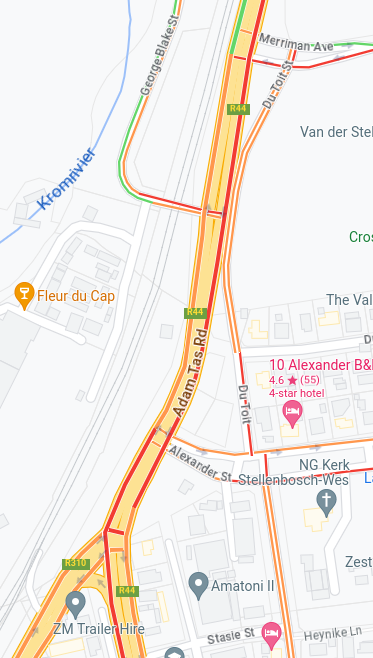
\includegraphics[scale = 0.75]{images/road.png}
\caption{\label{fig} The roads in question. Red shading indicated the slowest traffic, whereas green indicates the fastest. Data shows typical traffic on a Monday evening at 5 pm. Image credit: (Google, 2023a)}
\end{figure}

\section*{Phase 1: Simple model on a linear road segment}

\subsection*{The model}

For phase 1, the model stuck closely to the original proposal in (Nagel \& Schrekenberg, 1992), albeit with different boundary conditions that better reflect the reality of the road in question. In this model, a vehicle appears at the start(north) end of the road with a certain probability $q$ (provided the first cell is unoccupied). $p$ and $v$ have the same interpretation as in the original model, i.e. the probability of a vehicle randomly decelerating and the top speed for all vehicles respectively. The final variable is the length of the road $l$, in cells. The main observable of interest is the number of time-steps a vehicle spends on the road, on average (Time On Road or TOR).

\subsection*{Implementation}

This model was implemented in Java (see src/main/java/SimpleModel.java) this creates a class that can be instantiated using the four independent variables in the model at this phase: $q$, $p$, $v$ and $l$. One instantiated, the simulation can be run for single time-step at a time (using \texttt{step()}) or for any number of time-steps (using \texttt{run(int numSteps)}, which returns the average number of time-steps a vehicle spent on the road in that run).

To obtain some exploratory data, $1000$ simulations were run with values of $q \in \{0.1, \dots , 1\}$, $p \in \{0, \dots , 0.9\}$, $v \in \{3, 6, 9, 12\}$ and $l \in \{5, 10, 20, 40, 80\}$ for $10000$ time-steps, and TOR was recorded in (data/phase1/data.csv). This data was then analysed using numpy and matplotlib in dataAnalysis.ipynb. The coefficient of determination $r^{2}$ was calculated between every independent variable and TOR. For more detailed information, the coefficient of determination was also calculated for selected subsets of the data (e.g. only when $p$ is low). Plots were produced to show the relationship between TOR and some of the independent variables.

\subsection*{Results}

Unsurprisingly, the largest $r^{2}$ value was observed for $l$, the length of the road in cells, at 40.40\%. $p$ also had a significant effect on TOR, at 27.73\%. Interestingly, the overall effect of $q$ and $v$ was quite low, both with $r^{2}$ less than 1\% (0.8840\% and 0.9128\% respectively). For $p \leq 0.2$, $v$ had a slightly larger effect at 7.239\%. Conversely, $q$ has slightly more effect at higher $p$, 2.824\% for $p \geq 0.8$. Furthermore, when looking at low $p$ regimes, $r^{2}$ for $p$ itself is much lower, just 0.4989\% for $p \leq 0.2$ and 4.746\% for $p \leq 0.5$.

Since $l$ has such a dominating effect, observations were also made with $l$ fixed at 80. $p$ then became the dominating variable (58.70\%), with $v$ having a dominating effect when $p \leq 0.2$ (74.03\%) (fig. 3) and $q$ when $p \geq 0.8$ (73.57\%) (fig. 4).

\begin{figure}
\textbf{\large Average TOR as a function of $p$, with fixed $l=80$}\par\medskip
\rotatebox{90}{{\hspace*{3cm}{\large TOR}}}
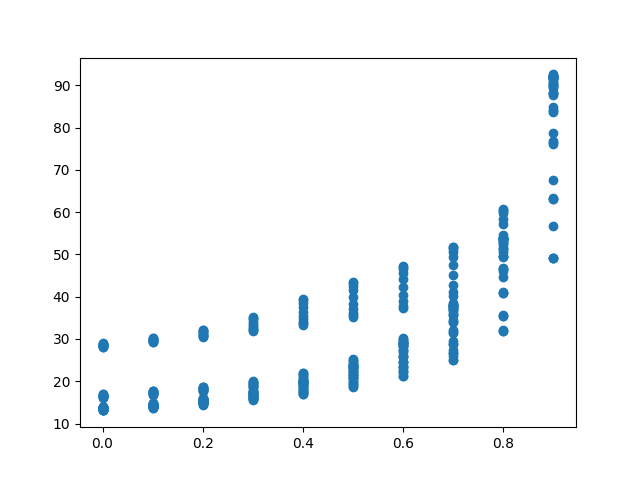
\includegraphics[scale = 0.55, left]{./data/phase1/p_vs_timeOnRoad_l=80.png}
\vspace*{0.1cm}\hspace*{4.5cm}{\large $p$}
\caption{\label{fig} With $l$ fixed at 80, TOR increases slowly with $p$ at first, but then grows exponentially as $p \to 1$.}
\end{figure}

\begin{figure}
\textbf{\large Average TOR as a function of $v$, with fixed $l=80$ and $p \leq 0.2$}\par\medskip
\rotatebox{90}{{\hspace*{3cm}{\large TOR}}}
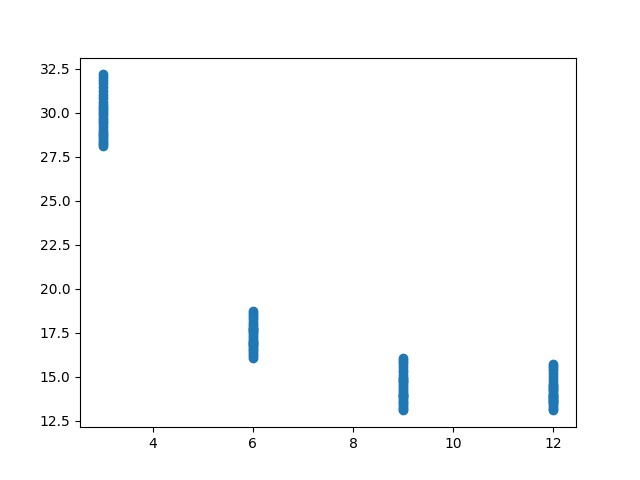
\includegraphics[scale = 0.55, left]{./data/phase1/v_vs_timeOnRoad_l=80_lowp.png}
\vspace*{0.1cm}\hspace*{4.5cm}{\large $v$}
\caption{\label{fig} Looking at low $p$ regimes, the effect of $v$ predominates, i.e. increasing $v$ reduces TOR significantly, albeit with diminishing returns.}
\end{figure}

\begin{figure}
\textbf{\large Average TOR as a function of $q$, with fixed $l=80$ and $p \geq 0.8$}\par\medskip
\rotatebox{90}{{\hspace*{3cm}{\large TOR}}}
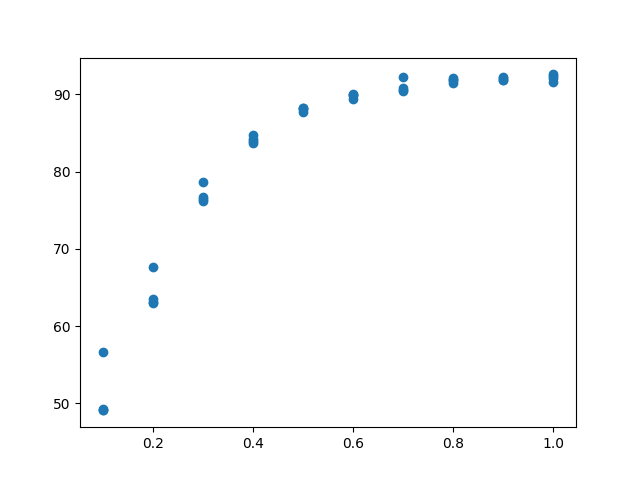
\includegraphics[scale = 0.55, left]{./data/phase1/q_vs_timeOnRoad_l=80_highp.png}
\vspace*{0.1cm}\hspace*{4.5cm}{\large $q$}
\caption{\label{fig} Looking at high $p$ regimes, the effect of $q$ predominates, i.e. more cars on the road slows things down regardless of top speeds.}
\end{figure}

\subsection*{Discussion}

As may be expected, these results indicate that the biggest factor by far influencing TOR is the length of the road. The top speed allowed on the road had a moderate effect when $p$ was low, and $p$ itself only had a large effect when it was quite high ($p \geq 0.5$, unlikely to occur in reality) (this is corroborated by the exponential-looking $p$-TOR curve, fig. 2). Somewhat surprisingly, the effect of $q$ was minimal, meaning that a busy road does not imply slow traffic in this model.

Removing $l$ changed this picture significantly, revealing two regimes at low and high $p$ respectively. When $p$ was low, $v$ determined TOR to a high degree, since vehicles were likely to actually reach the top speed when $p$ was low. However, $v$ was mostly irrelevant at high $p$, since vehicles are slowing down randomly too often to ever reach the top speed. In this regime, $q$ largely determined TOR, with a higher inflow of vehicles slowing traffic significantly.

\section*{Phase 2: Inflows and outflows via junctions}

\subsection*{The model}

In this phase, some of the variables had to be nailed down with real-world values to keep the size of the parameter space contained. The road segment in question is approximately 552 meters in length, and since a cell contains a single vehicle and (depending on exact conditions) perhaps 1 vehicle-length of following distance, the cell size was estimated at 7.5m which implies $l=74$. Estimating the average acceleration of vehicles on this road as $3m/s^{2}$, this means each time-step corresponds to approximately 2.5s in reality. Furthermore, this implies a maximum speed $v$ of 9 (27 m/s = 97.2 km/h--the true speed limit is 100km/h).

To model the junctions themselves, six more variables were introduced, two for each of the three junctions, namely the probability of a vehicle leaving/joining the R44 at that junction. Vehicles join the R44 simply by appearing at the position of the junction. To be slightly more realistic, the leaving process is somewhat more complex. First, vehicles that will reach/pass a particular junction are identified, and a portion of them are randomly assigned to turn off at the junction according to the leaving probability. These then slow down to reach one cell before the junction by the end of this time-step. Finally, these vehicles "turn off" (i.e. disappear from the model) during the next time-step.

At this point, the model still had 8 variables, all of which could vary independently and continuously between 0 and 1 (since they are all probabilities of some kind). Limiting the range of some of these to values that are physically realistic was therefore necessary to investigate the behaviour effectively. Extrapolating from existing data on traffic flow collected in 2018 (Bredenhann, 2022), reasonable estimates can be made for many of these variables (see table below).

\begin{center}
\begin{tabular}{ |c|c|c| }
 \hline
 Junction & Direction & Probability \\
 \hline
 R44 (i.e. already on road) & Incoming & 0.7736\\
 Merriman & Incoming & 0.7132 \\
 Merriman & Outgoing & 0.3139 \\
 George Blake & Incoming & 0.3938 \\
 George Blake & Outgoing & 0.4007 \\
 Alexander & Incoming & 0.4725 \\
 Alexander & Outgoing & 0.1640 \\
 \hline
\end{tabular}
\end{center}

Data for Alexander Street was not available in (Bredenhann, 2022), so data was collected on the evening of Friday 3 November from 16:20 until around 17:10. Control data was also collected for incoming vehicles on the north end of the R44 so an adjustment could be made for presumed lower traffic volumes on Fridays, and due to the relative dearth of student drivers during the exam period. Traffic flow on the R44 was 85.10\% of those recorded in (Bredenhann, 2022), so volumes recorded on Alexander Street were accordingly multiplied by a factor of 1.175.

Finally, using TOR as a metric in this phase would be complicated by the fact that vehicles coming in from different junctions have different lengths of road to cover, and lumping them all together would not yield any insightful results. Therefore, the average speed would be the main metric of interest, from which TOR from each junction can be estimated.

\subsection*{Implementation}

This model was implemented in the \texttt{JunctionModel} class, which is a subclass of \texttt{SimpleModel} used for phase 1. Fields were added for the inflow and outflow probabilities as indicated in the table above, with $v$ and $l$ now fixed to correspond to their real-world values. Furthermore, the \texttt{step()} function had to be updated to mark vehicles that will leave the road at the next junction (which necessitated a \texttt{destination} field to be added to the \texttt{Vehicle} class) and to remove these when they reached the junction in question. \texttt{run(int numSteps)} was also updated to record average speeds instead of TOR.

1000 simulations were run for 1440 time-steps each (corresponding to 1 hour in real-world time) for each $p \in \{0, 0.01, \dots , 0.99\}$ and the average speed recorded in data/phase2/data.csv. This data was then used in dataAnalysis.ipynb to create a plot of $\langle v \rangle$ as a function of $p$.

\subsection*{Results}

Average speeds were on the low end, reflecting real-world traffic conditions. In the ideal case, when $p=0$, speeds reached $v=1.178$, corresponding to a real-world 12.72km/h, degenerating to $v=0$ when $p=1$ and no vehicle ever moves.

Google maps predicts travel times on the entire stretch from just above Merriman to the R310 to be "typically 3-7 minutes" at 5pm on a Tuesday evening (ie. evening peak hours)(Google 2023b). Combined with the data generated here, this can be used to estimate $p$ on this road segment.

A travel time of 3 minutes implies an average speed of $v=1.022$ and 7 minutes $v=0.4381$, which correspond to $p=0.08$ and $p=0.62$ respectively. The median travel time of 5 minutes corresponds approximately to $p=0.31$.

\begin{figure}
\textbf{\large Average speed as a function of $p$}\par\medskip
\rotatebox{90}{{\hspace*{3cm}{\large $\langle v \rangle$}}}
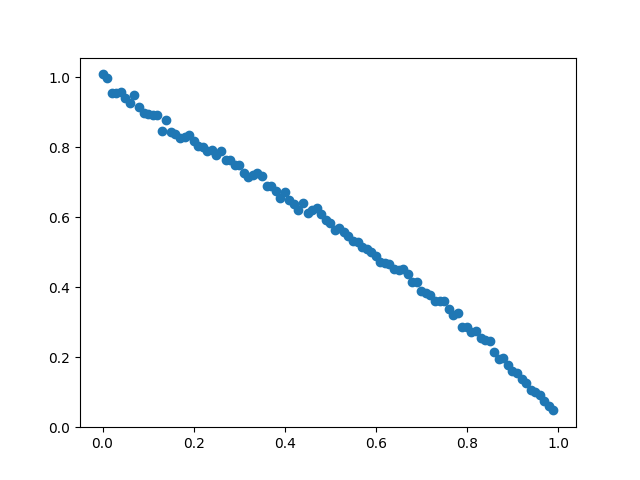
\includegraphics[scale = 0.55, left]{./data/phase2/v_vs_p.png}
\vspace*{0.1cm}\hspace*{4.5cm}{\large $p$}
\caption{\label{fig} Average speeds are low overall due to high congestion, but are even lower at high $p$.}
\end{figure}

\section*{Phase 3: Traffic lights}

\subsection*{The model}

In this phase, the model was improved by the addition of traffic lights regulating flow at junctions. Traffic lights are modelled to all be identical, being red half the time and green the other half, switching between these states every $t$ time-steps. The main goal of this phase was to investigate the effect this $t$ has at various values of $p$. Given the results of phase 2, $p$ was restricted to $[0.05, 0.65)$. $t$ was taken between 1---2.5s, hardly enough time for even one vehicle to cross---to 120---5 minutes, longer than most road users would find acceptable.

\subsection*{Implementation}

This phase of the model was implemented in the \texttt{TrafficLightModel} class, a subclass of \texttt{JunctionModel}. Incoming vehicles from junctions were added to queues (specifically, the in-built \texttt{ArrayBlockingQueue<Vehicle>}), waiting for the light to turn green to allow them onto the R44. The \texttt{step()} function was updated to include slowing down for the traffic lights, and the lights themselves were encapsulated in the \texttt{TrafficLight} class, which included the functions \texttt{check()} to determine if the light is red or green, \texttt{incrementTime()} to move the traffic light along one time-step, and \texttt{change()} to change the traffic light from red to blue and vice versa.

Average speeds on the R44 itself and average lengths of all queues over 1000 runs were recorded in data/phase2/data.csv for $t \in \{1, 2, \dots , 120\}$ and $p \in \{0.05, 0.1, \dots , 0.65\}$. This data was used in dataAnalysis.ipynb to produce plots of $\langle v \rangle$ and queue length as a function of $t$ for each value of $p$.

\subsection*{Results}

Results differed quantitatively for different $p$, but always following a similar pattern: slow average speeds when $t$ is small and vehicles have to stop at junctions all the time, a peak somewhere between $t=22$ (when $p=0.05$) and $t=40$ (when $p=0.6$), and then tailing off for larger $t$ with vehicles having to wait for long periods. Some graphs of $\langle v \rangle$ versus $t$ for selected $p$ are shown in figs. 6-9.

\begin{figure}
\textbf{\large Average speed as a function of $t$ at $p=0.05$}\par\medskip
\rotatebox{90}{{\hspace*{3cm}{\large $\langle v \rangle$}}}
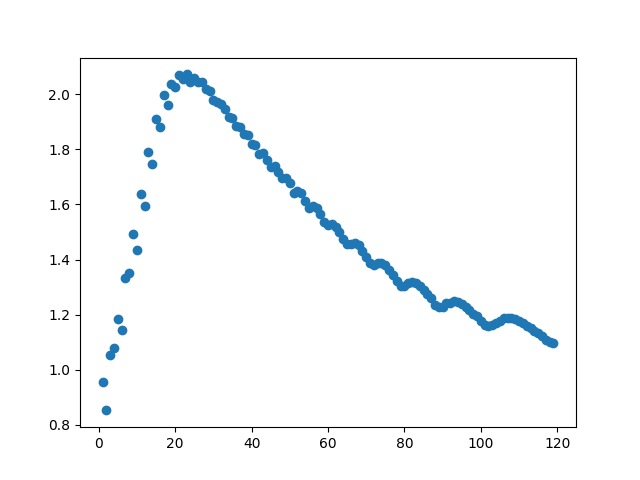
\includegraphics[scale = 0.55, left]{./data/phase3/v_vs_t_p=0.05.png}
\vspace*{0.1cm}\hspace*{4.5cm}{\large $t$}
\caption{\label{fig} At the lowest $p$ considered in this phase, $\langle v \rangle$ peaks at $t=22$, meaning the traffic light changes state every 55 seconds}
\end{figure}

\begin{figure}
\textbf{\large Average speed as a function of $t$ at $p=0.15$}\par\medskip
\rotatebox{90}{{\hspace*{3cm}{\large $\langle v \rangle$}}}
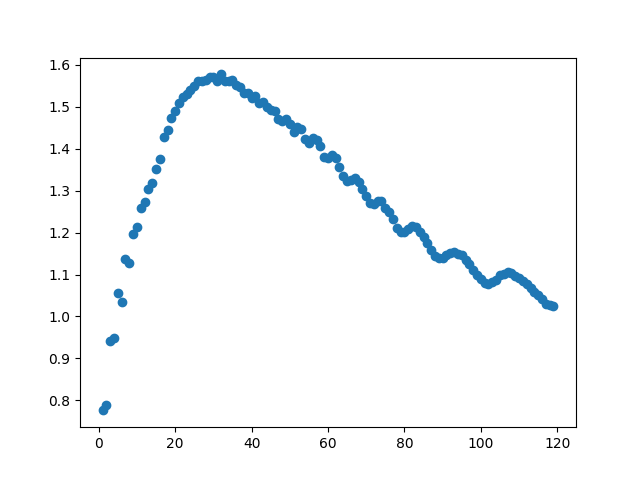
\includegraphics[scale = 0.55, left]{./data/phase3/v_vs_t_p=0.15.png}
\vspace*{0.1cm}\hspace*{4.5cm}{\large $t$}
\caption{\label{fig} At the lowest $p$ considered in this phase, $\langle v \rangle$ peaks at $t=31$, meaning the traffic light changes state every 77.5 seconds}
\end{figure}

\begin{figure}
\textbf{\large Average speed as a function of $t$ at $p=0.3$}\par\medskip
\rotatebox{90}{{\hspace*{3cm}{\large $\langle v \rangle$}}}
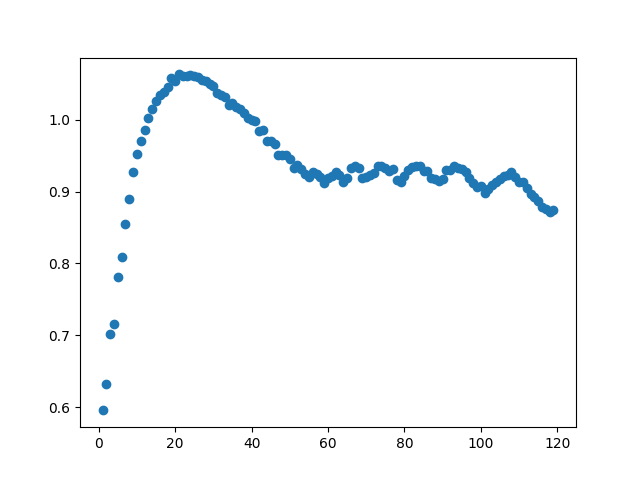
\includegraphics[scale = 0.55, left]{./data/phase3/v_vs_t_p=0.3.png}
\vspace*{0.1cm}\hspace*{4.5cm}{\large $t$}
\caption{\label{fig} At the lowest $p$ considered in this phase, $\langle v \rangle$ peaks at $t=27$, meaning the traffic light changes state every 67.5 seconds}
\end{figure}

\begin{figure}
\textbf{\large Average speed as a function of $t$ at $p=0.6$}\par\medskip
\rotatebox{90}{{\hspace*{3cm}{\large $\langle v \rangle$}}}
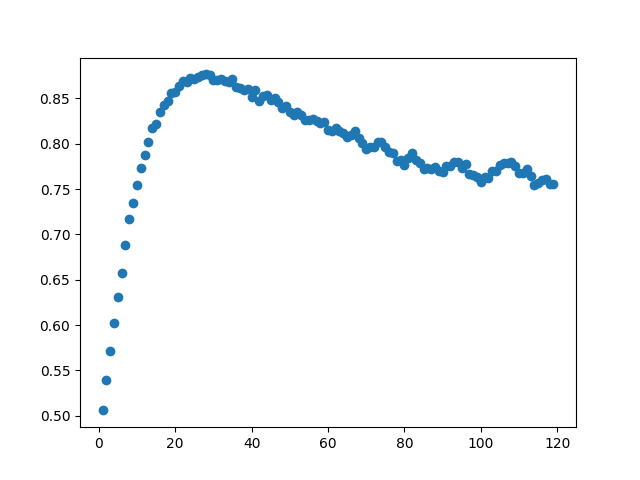
\includegraphics[scale = 0.55, left]{./data/phase3/v_vs_t_p=0.6.png}
\vspace*{0.1cm}\hspace*{4.5cm}{\large $t$}
\caption{\label{fig} At the lowest $p$ considered in this phase, $\langle v \rangle$ peaks at $t=40$, meaning the traffic light changes state every 100 seconds}
\end{figure}

Average queue lengths did not differ much for different $p$, so fig. 10 is representative.

\begin{figure}
\textbf{\large Average queue lengths of $t$ at $p=0.3$}\par\medskip
\rotatebox{90}{{\hspace*{3cm}{\large Queue length (vehicles)}}}
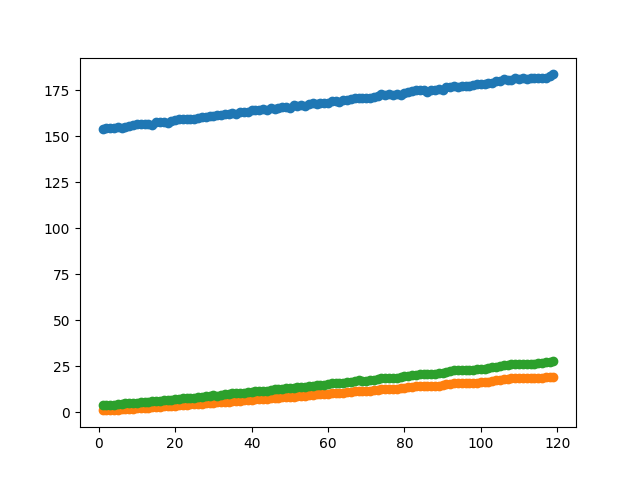
\includegraphics[scale = 0.55, left]{./data/phase3/queue_lengths_vs_t_p=0.3.png}
\vspace*{0.1cm}\hspace*{4.5cm}{\large $t$}
\caption{\label{fig} Average queue lengths as a function of $t$. Blue represents Merriman, orange George Blake, and green Alexander Street}
\end{figure}

\subsection*{Discussion}

It is interesting to note that 1. for some $t$, average speeds were significantly faster than those recorded in phase 2 for the same $p$, and 2. the wavy pattern shown at high $t$ in figs. 6-9. The first of these can be explained by the fact that in phase 2, vehicles entered the road willy-nilly at an initial speed of 0, constantly causing all traffic to slow down. In phase 3, however, vehicles can move unimpeded half the time, when the traffic lights are green.

Explaining the second phenomenon is a bit more tricky, however. It is clear that the waves increase in intensity and period as $t$ increases (except possibly at higher $p$---the data is a bit too noisy there to be certain), but this does not point to any particular cause. One possible explanation is a kind of "harmonic" effect, where $\langle v \rangle$ is higher at values near particular multiples of the peak $t$. Another possibility is that these values of $t$ allow vehicles with a particular (and probable) initial speed to move all the way through this road segment with no stopping whereas nearby values of $t$ do not. Ultimately, while interesting, this phenomenon falls outside the scope of this study and was not investigated extensively.

\section*{Phase 4: Parallel traffic flow in Du Toit Street}

\subsection*{The model}

Conceptually, phase 4 is another fairly minor evolution of its predecessor. Vehicles on Merriman waiting to enter the R44 can make their way down Du Toit Street instead and bypass a lot of traffic by joining the R44 at Alexander Street. This adds a third variable to the equation, $d$, the probability that a vehicle waiting on Merriman Avenue takes this detour. To assess this strategy, two factors will be considered: whether the vehicles taking the detour indeed reach their destination faster, and any effect taking the detour may have on overall flow of traffic.

It stands to reason that $p$ and $t$ should not change too much from one evening to the next, so, to simplify things, these were fixed to particular values for this phase. The data collected for Alexander Street also included timings on traffic lights, which averaged around 30-40 seconds between every state change, depending on traffic conditions. This corresponds to $12 \leq t \leq 16$, noticeably lower than the values that produced the highest $\langle v \rangle$ in phase 3. The average value of $t=14$ was fixed for this phase. Given the findings in phase 2, $p$ was also fixed to 0.3.

\subsection*{Implementation}

This phase was implemented mainly in the \texttt{FinalModel} class, a subclass of \texttt{TrafficLightModel}, with the \texttt{DuToitModel} class (a subclass of \texttt{SimpleModel}) as a singleton to model Du Toit Street specifically therein. The \texttt{step()} function of \texttt{FinalModel} was modified to allow vehicles in the Merriman queue to enter Du Toit Street based on the detour probability $d$, and to join the Alexander queue when reaching the end of Du Toit Street, as well as adding fields for tracking TOR from Merriman via both routes. The only change to \texttt{DuToitModel} compared to its superclass was vehicles slowing down when reaching the end of the road and waiting to be scooped up by the \texttt{FinalModel} that placed them in the Alexander Street queue.

The \texttt{Vehicle} class was modified to track the origins of vehicles, since we are only really interested in vehicles from Merriman Avenue for this phase, as well as the route they followed (i.e. whether they went straight into the R44 or via Du Toit Street) for comparison purposes.

\subsection*{Results}

Somewhat surprisingly, taking the detour down Du Toit Street was never significantly faster than going down the R44 (fig. 11). For very low $d$ Du Toit Street was marginally faster, but by $d = 0.06$ the R44 was faster and the difference becomes quite stark very quickly at moderate to high $d$. Part of the reason for this may be seen in fig. 12. For $d < 0.14$, the Merriman queue is the longest and causes the most delay, so any transfers to the Alexander queue relieves this pressure and speeds things up. However, when $d \geq 0.14$, the Alexander queue is the longest, so trying to transfer to it from Merriman is counterproductive since you will spend longer waiting there.

Furthermore, vehicles turn into Du Toit Street from the head of the Merriman queue (in the simulation at least, in reality the two junctions are a few metres apart) which means that vehicles taking the detour had to wait in the Merriman queue anyway---which is why the two lines in fig. 11 follow a similar trajectory for very low $d$ before diverging.

Ironically, however, taking the Du Toit Street bypass lowers congestion on the R44 itself and shortens the queue to enter from Merriman Avenue, increasing average speeds and making journeys faster for everyone else (except those who wanted to enter from Alexander Street originally). These faster journey times can be seen in fig. 11, and on the graph of average speeds shown in fig. 13.

\begin{figure}
\textbf{\large Average TOR as a function of $d$}\par\medskip
\rotatebox{90}{{\hspace*{3cm}{\large TOR}}}
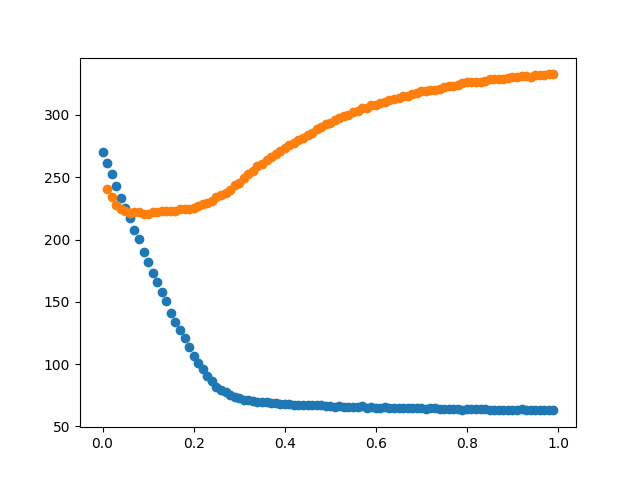
\includegraphics[scale = 0.55, left]{./data/phase4/TORs_vs_d.png}
\vspace*{0.1cm}\hspace*{4.5cm}{\large $d$}
\caption{\label{fig} TOR from Merriman to the R310 as a function of $d$. Blue represents vehicles that stick to the R44, and orange those that use the Du Toit Street bypass}
\end{figure}

\begin{figure}
\textbf{\large Average queue length as a function of $d$}\par\medskip
\rotatebox{90}{{\hspace*{3cm}{\large Queue length (vehicles)}}}
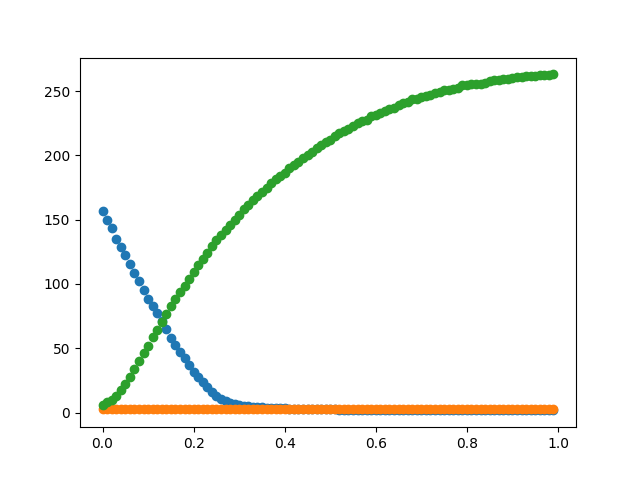
\includegraphics[scale = 0.55, left]{./data/phase4/queues_vs_d.png}
\vspace*{0.1cm}\hspace*{4.5cm}{\large $d$}
\caption{\label{fig} Average queue lengths waiting to enter the R44 as a funtion of $d$. Blue represents Merriman, orange George Blake, and green Alexander Street}
\end{figure}

\begin{figure}
\textbf{\large Average speed on the R44 as a function of $d$}\par\medskip
\rotatebox{90}{{\hspace*{3cm}{\large $\langle v \rangle$}}}
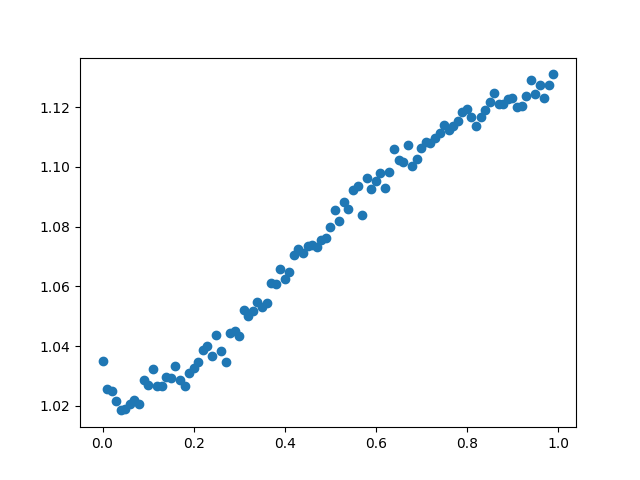
\includegraphics[scale = 0.55, left]{./data/phase4/v_vs_d.png}
\vspace*{0.1cm}\hspace*{4.5cm}{\large $d$}
\caption{\label{fig} Average speeds on the R44 as a function of $d$}
\end{figure}

\section*{Conclusion}

The main finding was that using the Du Toit Street bypass is not an effective way to decrease journey times between Merriman Avenue and the R310, and in fact is significantly slower in most situations. Possible limitations on this finding include variability in how long traffic lights are red/green, traffic conditions changing at different times of the day or year, potential variability in the value of $p$, and the presence of trucks and other large vehicles with lower acceleration that effectively occupy multiple "cells", all of which were not taken into account here. It is also possible that some of the assumptions made re. cell size, acceleration, etc. may simply not be realistic.

A secondary finding was that traffic lights change more often than the model would suggest is optimal, which points to the most important caveat: people making their way home after a long day's work are impatient, and they would rather have a sense of constantly moving forward than long waits that technically minimise their overall travel time. Furthermore, some drivers may make irrational decisions in situations such as these simply because it gives them something to do rather than simply waiting for a light to turn green.

\pagebreak

\section*{References}

Bredenhann, C. (2022). \textit{Stellenbosch Municipality Roads Master Plan: 2022 update}.

Google. (2023a). Retrieved 25 October 2023 from https://www.google.com/maps/@-33.9354554,18.8545061,17z/data=!5m1!1e1?entry=ttu

Google. (2023b). Retrieved 31 October 2023 from https://www.google.com/maps/dir/-33.9325783,18.8529169/-33.9371228,18.8515087/@-33.9349965,18.8496809,17z/data=
!4m6!4m5!2m3!6e0!7e2!8j1698771600!3e0?entry=ttu

Nagel, K.; Schreckenberg, M. (1992). "A cellular automaton model for freeway traffic". \textit{Journal de Physique I} 2(12) doi:10.1051/jp1:1992277

\end{document}